\documentclass[
size=17pt,
paper=smartboard,
mode=present,
display=slidesnotes,
style=paintings,
nopagebreaks,
blackslide,
fleqn]{powerdot}

% styles: sailor, paintings
% wj capsules prettybox
% mode = handout or present


\usepackage{amsmath,graphicx,color,amsfonts}
\usepackage[brazilian]{babel}
\usepackage[ruled,vlined,portuguese,portuguesekw]{algorithm2e}
\usepackage[utf8]{inputenc}
\newcommand{\palette}{Moitessier}


% palettes:
%    - sailor: Sea, River, Wine, Chocolate, Cocktail 
%    - paintings: Syndics, Skater, GoldenGate, Moitessier, PearlEarring, Lamentation, HolyWood, Europa, MayThird, Charon 

\newcommand{\cursopequeno}{EC01039 CG\underline{PI}}
\newcommand{\cursogrande}{\Large EC01039 -- Computação gráfica e \underline{processamento de imagem}}



\author{Ronaldo de Freitas Zampolo\\FCT-ITEC-UFPA}
\date{ERE 2020}


\pdsetup{
	lf = {\cursopequeno},
	rf = {Transformações de intensidade}, 
	cf = {\arabic{slide}~/~\pageref*{lastslide}},
	palette = {\palette}, 
	randomdots={false}
}

%opening
\title{\cursogrande\\ \vspace{1cm}Transformações de intensidade}
\author{Ronaldo de Freitas Zampolo\\FCT-ITEC-UFPA}
%\date{ }

\begin{document}
   \maketitle[randomdots={false}]
   \begin{slide}{Agenda}
      \tableofcontents[content=sections]
   \end{slide}

\section[ slide = true ]{Fundamentos}
      \begin{slide}[toc=]{Introdução}
         \begin{itemize}[type=1]
            \item Técnicas que manipulam diretamente os pixels de uma imagem
            \item Transformação de intensidade: mapeamento entre níveis de cinza (ponto a ponto)
            \begin{equation*}
               g(x,y) = T\left [ f(x,y)\right ]
            \end{equation*}
            \begin{center}
              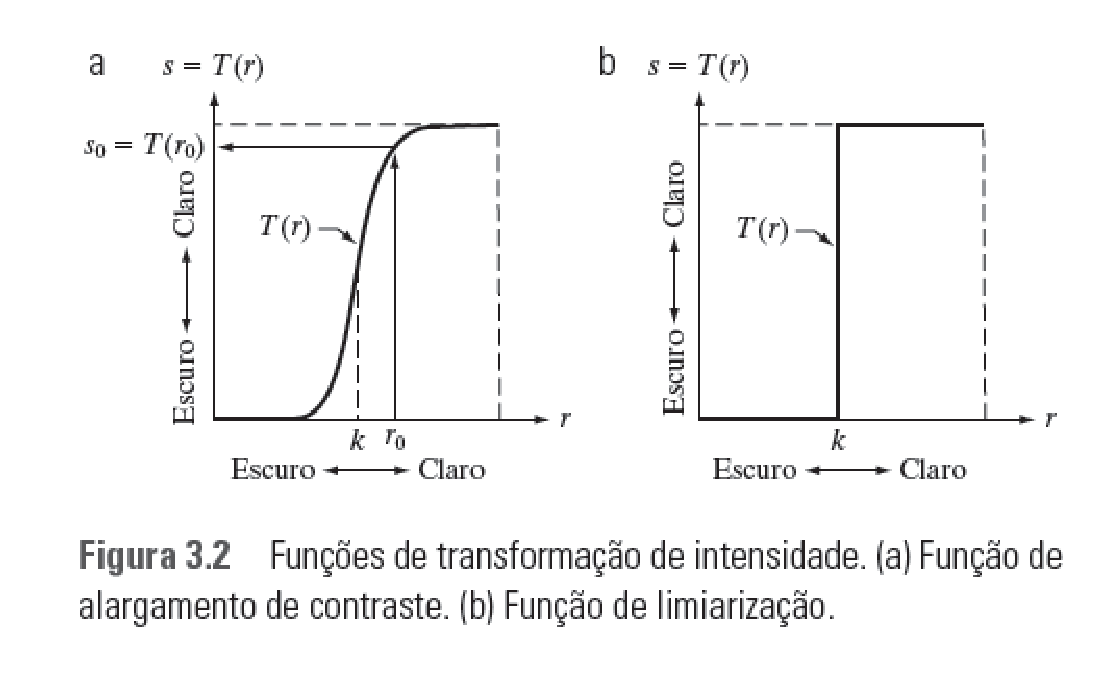
\includegraphics[width=0.55\textwidth]{figs/fig0302}
           \end{center}
         \end{itemize}
      \end{slide}

       \begin{slide}[toc=]{Introdução}
          \twocolumn{
          \begin{itemize}[type=1]
             \item Filtragem: processamento por vizinhança
            \begin{itemize}
               \item Caso o sistema seja linear e invariante: mapeamento entre entrada e saída é dado pela convolução bidimensional
               \begin{align*}
                  g(x,y) &= h(x,y)\ast f(x,y)\\
                         &= \sum_{s=-a}^{a}\sum_{t= -b}^{b} f(s,t)h(x-s,y-t) 
               \end{align*} 
           \end{itemize}
          \end{itemize}
           }{
             \begin{center}
                 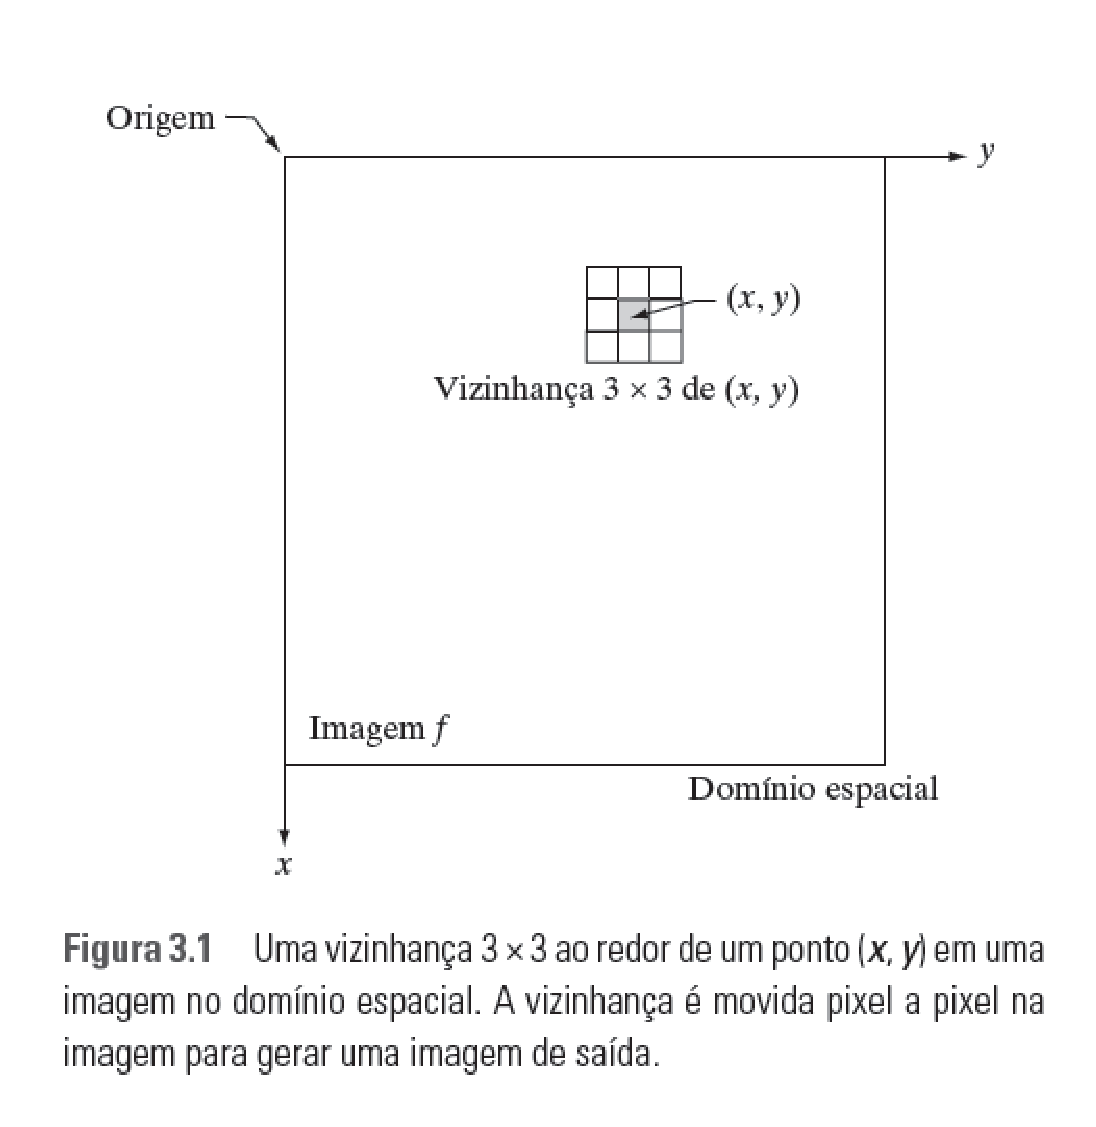
\includegraphics[width=0.9\textwidth]{figs/fig0301}
              \end{center}
              }

       \end{slide}

   \section[ slide = true ]{Transformação de intensidade}
      \begin{slide}[toc=]{Funções básicas}
         \begin{itemize}[type=1]
          \item Algumas transformações básicas
          \begin{center}
                  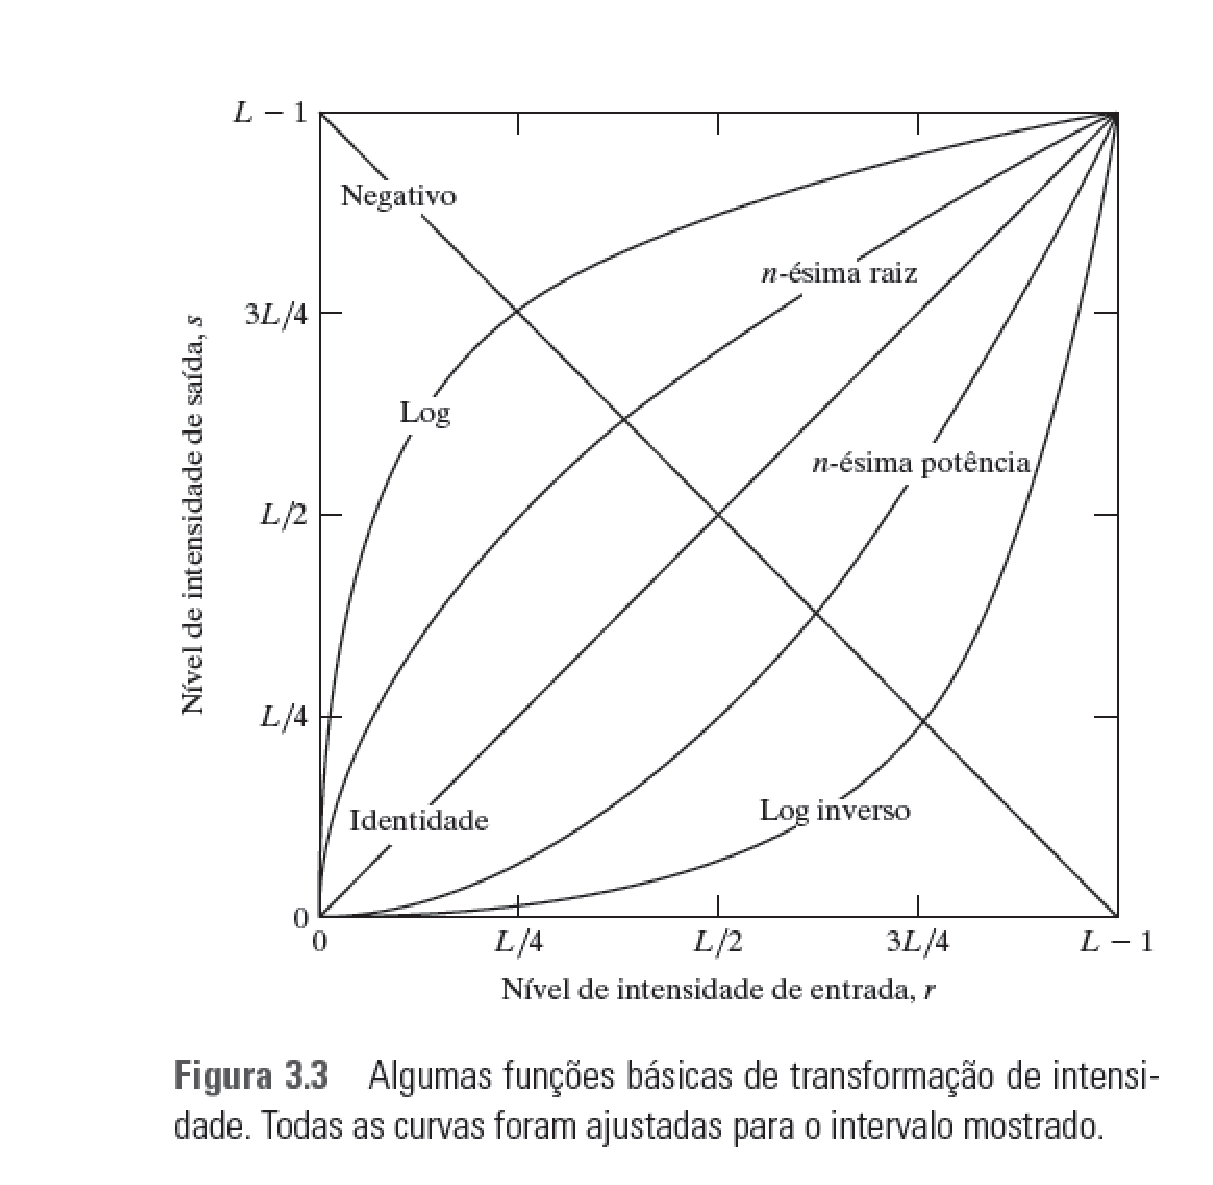
\includegraphics[width=0.5\textwidth]{figs/fig0303}
               \end{center}
         \end{itemize}
      \end{slide}

       
      \begin{slide}[toc=]{Funções básicas}
         \begin{itemize}[type=1]
            \item Negativo da imagem
            \begin{itemize}
               \item Intervalo de níveis de cinza: $[0,L-1]$
               \item Relação entre entrada e saída: \begin{equation*}g(x,y) = L-1 - f(x,y)\end{equation*}
               \begin{center}
                  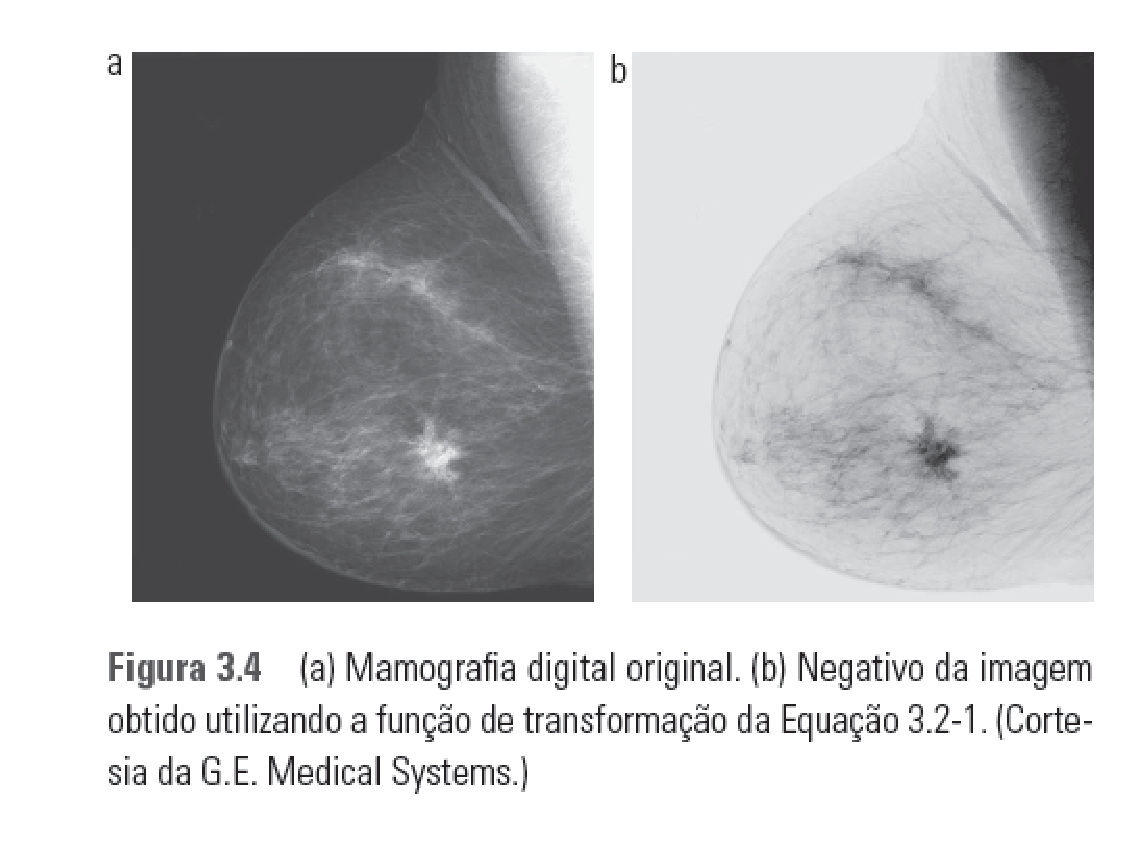
\includegraphics[width=0.45\textwidth]{figs/fig0304}
               \end{center}
            \end{itemize}
         \end{itemize}
         
      \end{slide}
            
     \begin{slide}[toc=]{Funções básicas}
         \begin{itemize}[type=1]
            \item Transformações logarítmicas 
            \begin{itemize}
               \item Relação entre entrada e saída: \begin{equation*}g(x,y) = k\log\left [1+f(x,y)\right ]\end{equation*}
               \item Parâmetro $k$: constante 
               \item $f(x,y)\geq 0$
            \end{itemize}
         \end{itemize}         
      \end{slide}
   
      \begin{slide}[toc=]{Funções básicas}
         
         \begin{itemize}[type=1]
            \item Transformações de potência 
            \begin{itemize}
               \item Relação entre entrada e saída: \begin{equation*}g(x,y) = \begin{cases}
                                                                               k\left [f(x,y)\right ]^\gamma\\
                                                                               k\left [f(x,y)+\varepsilon\right ]^\gamma

                                                                              \end{cases}
                                                    \end{equation*}
               \item Constantes positivas: $k$ e $\gamma$
               \item Offset: $\varepsilon$
            \end{itemize}
         \end{itemize}
      \end{slide}
         
      \begin{slide}[toc=]{Funções básicas}
      \begin{itemize}
       \item Variação da função de mapeamento com $\gamma$
      \end{itemize}

         \begin{center}
                  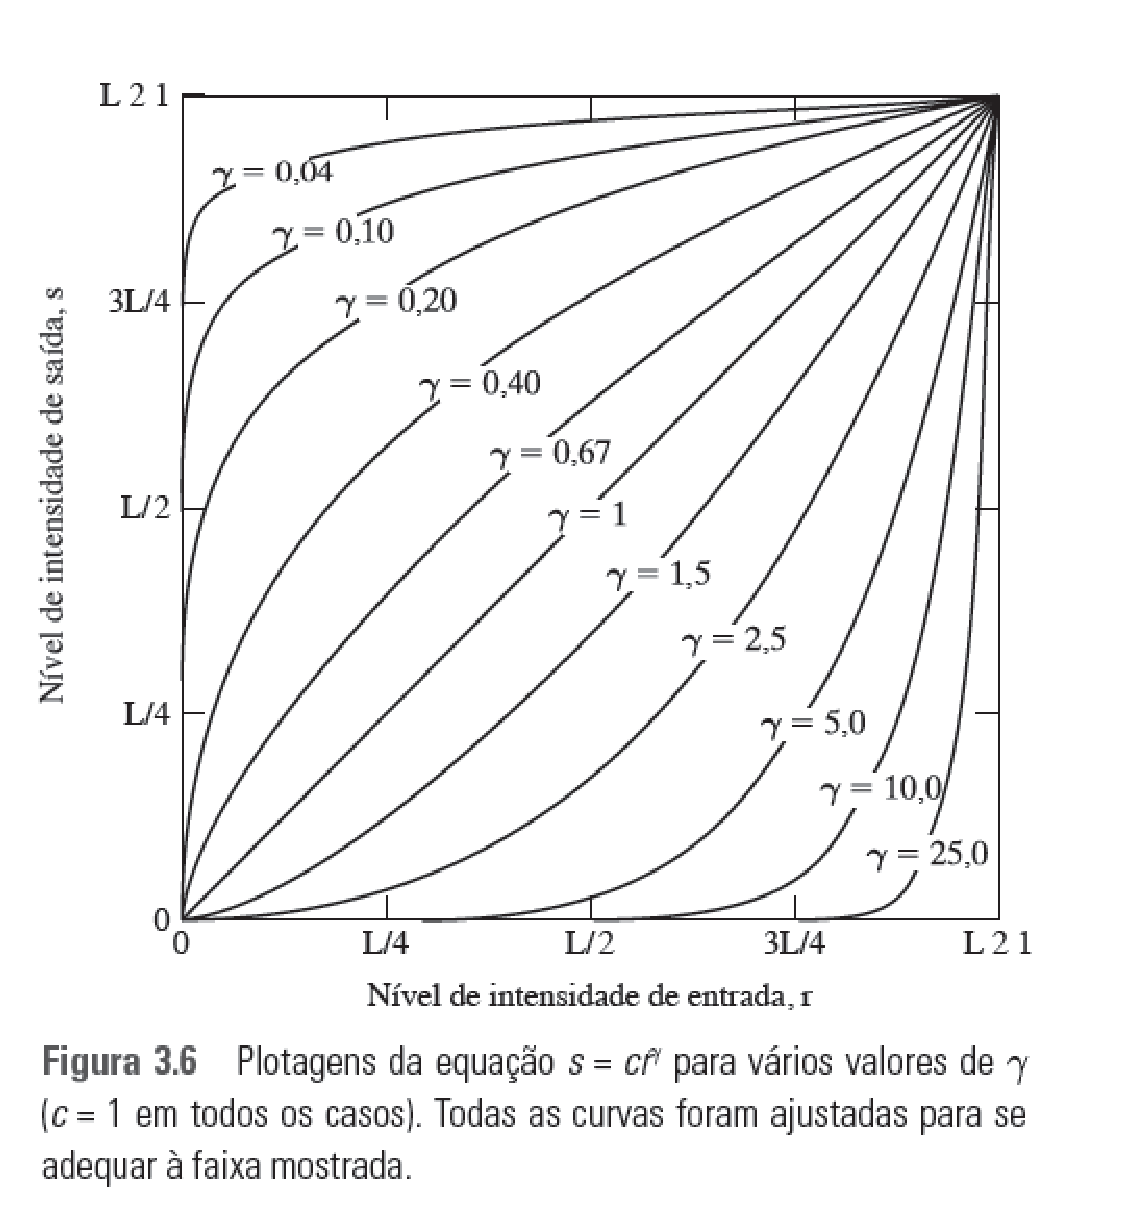
\includegraphics[width=0.4\textwidth]{figs/fig0306}
               \end{center}
         
       \end{slide}
       
      \begin{slide}[toc=]{Funções básicas}
      \begin{itemize}
       \item Correção gama: exemplo
      \end{itemize}
         \begin{center}
                  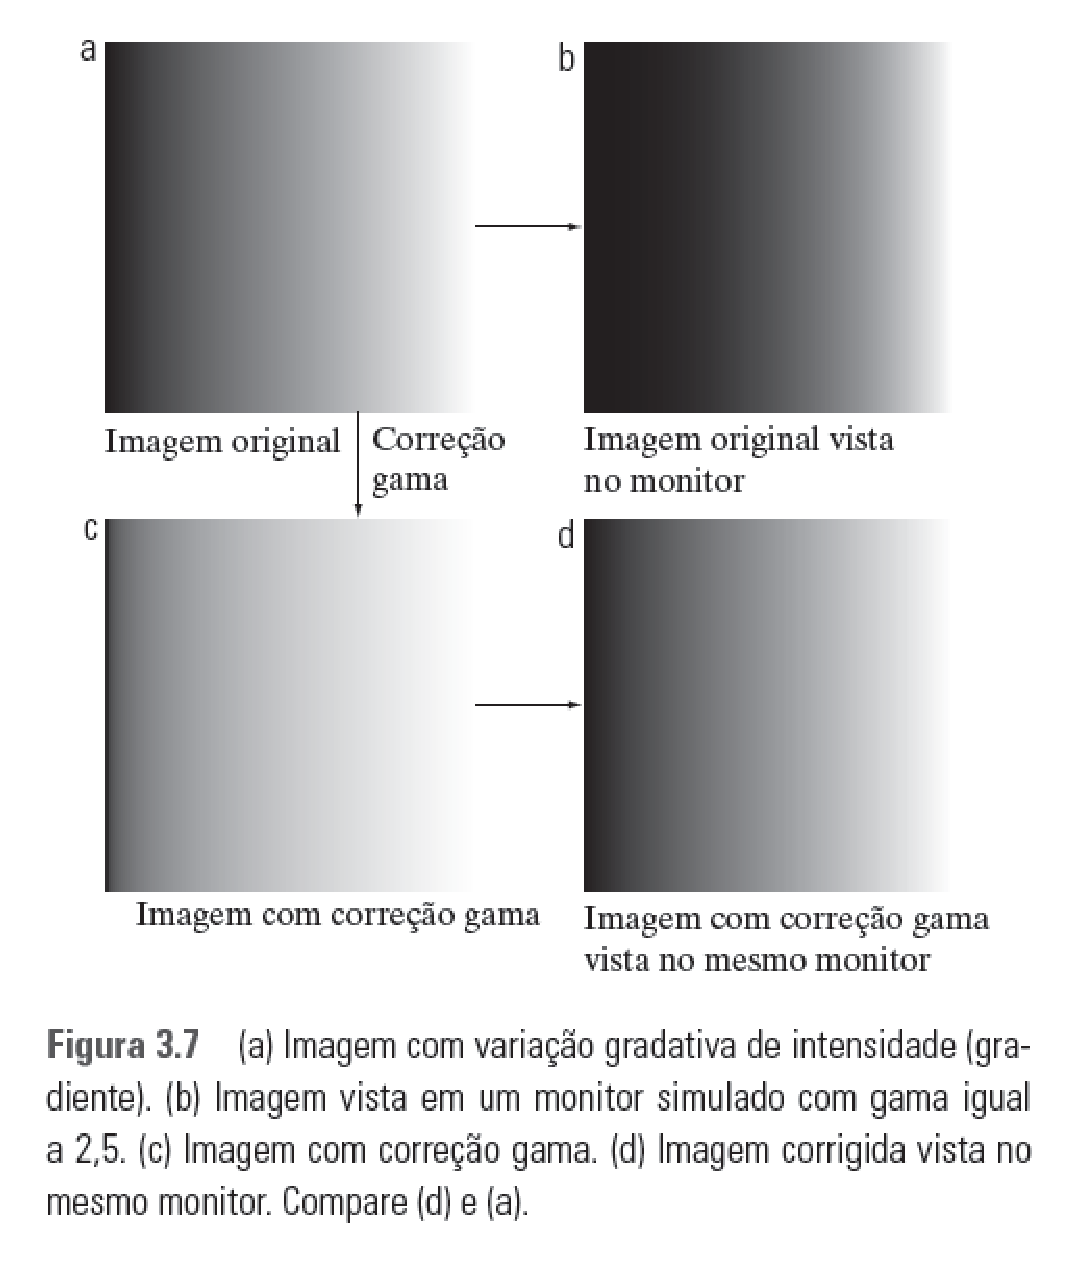
\includegraphics[width=0.4\textwidth]{figs/fig0307}
               \end{center}
         
       \end{slide}
       
       \begin{slide}[toc=]{Funções básicas}
      \begin{itemize}
       \item Mais um exemplo
      \end{itemize}
         \begin{center}
                  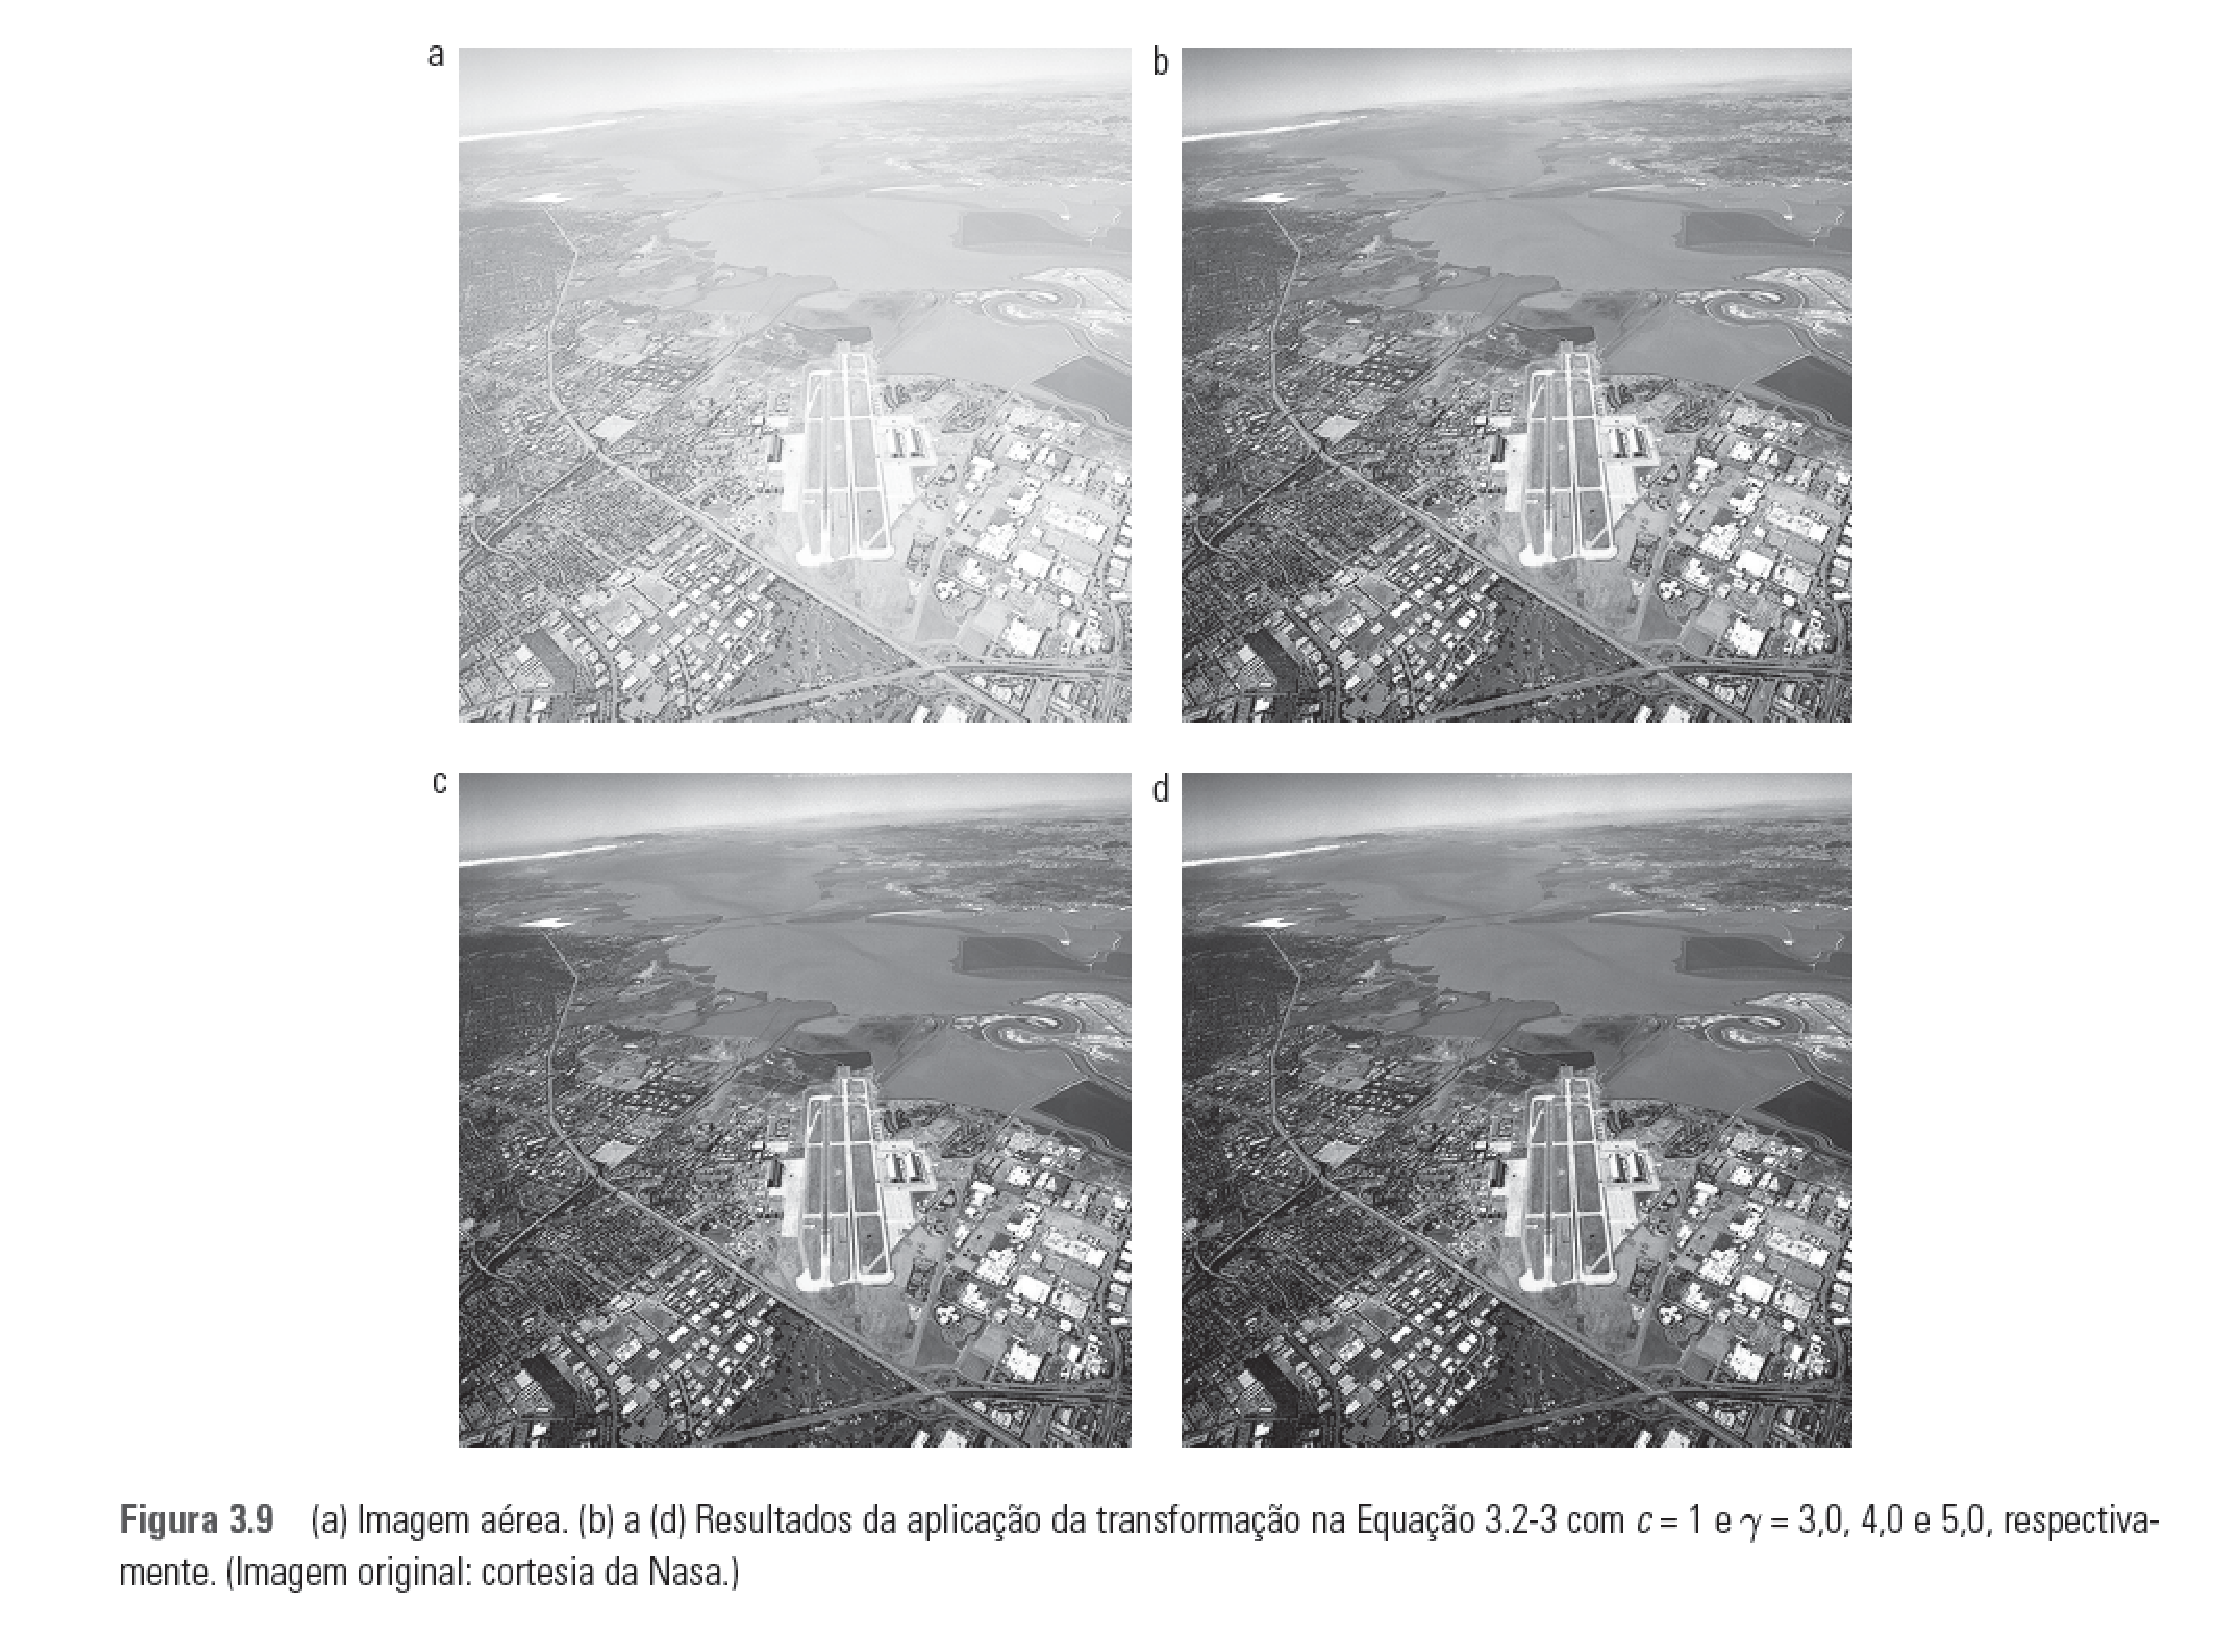
\includegraphics[height=0.65\textheight]{figs/fig0309}
               \end{center}
         
       \end{slide}
       
   \begin{slide}[toc=]{Outras funções de transformação}
      \begin{itemize}
         \item Liberdade na definição de funções
      \end{itemize}
         \begin{center}
             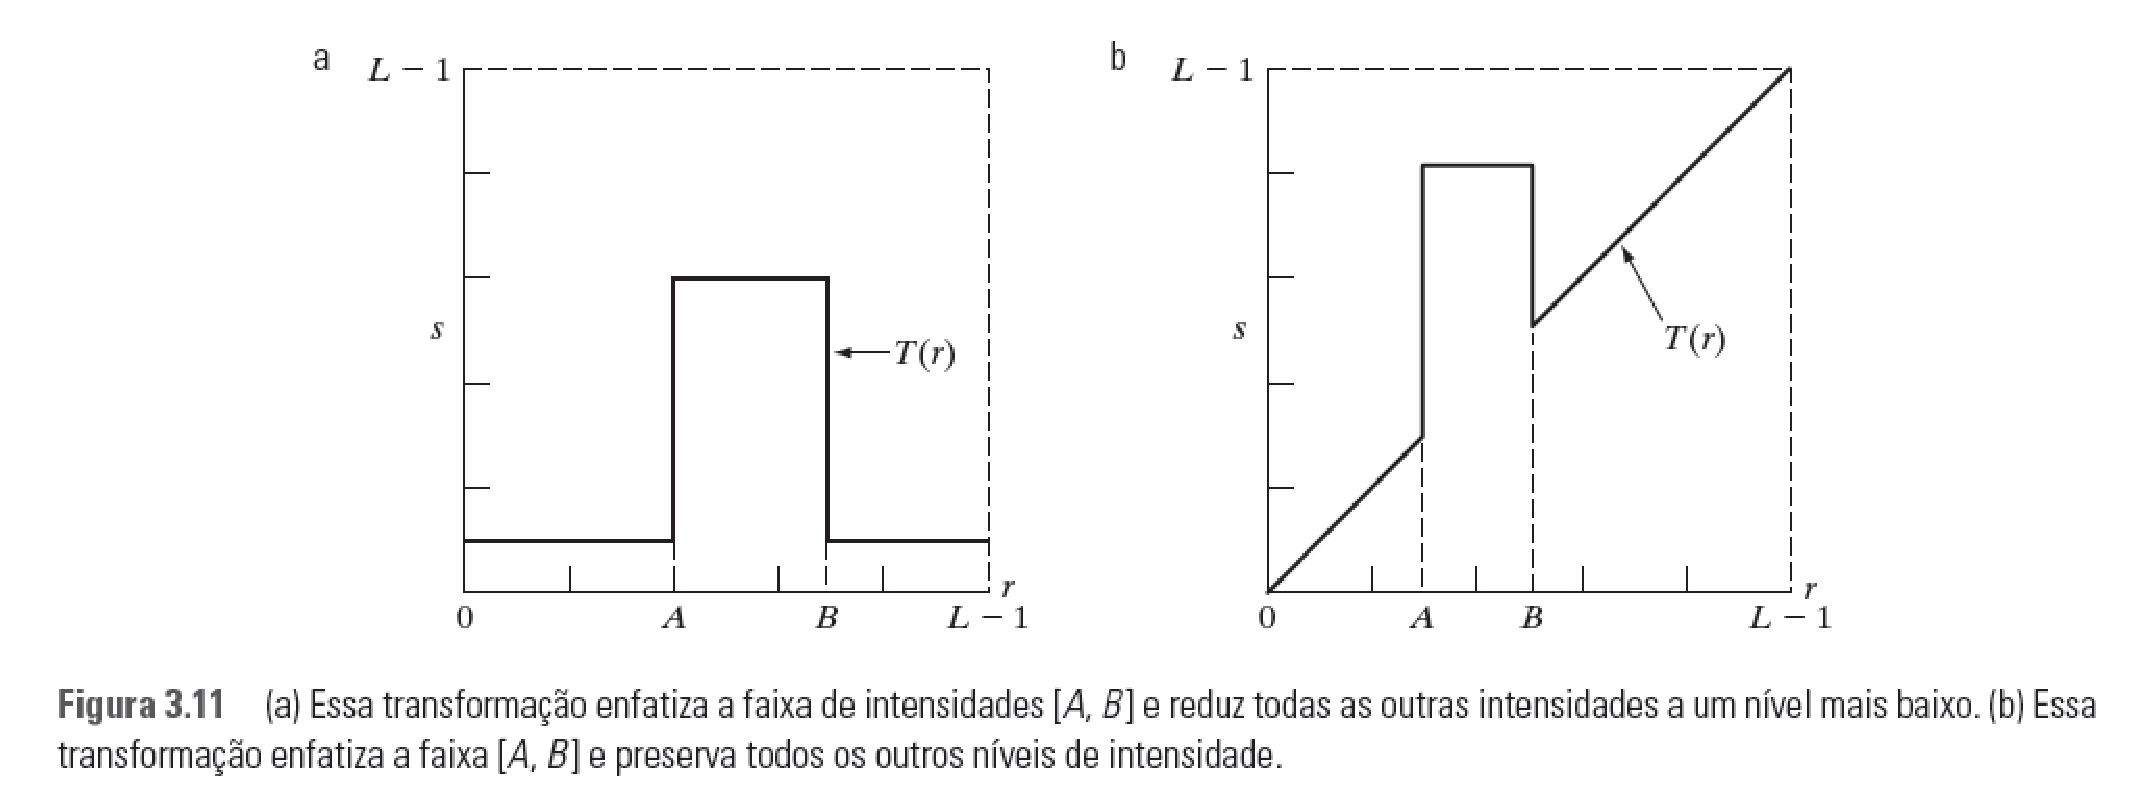
\includegraphics[width=\textwidth]{figs/fig0311}
         \end{center}
    \end{slide}

   \begin{slide}[toc=]{Outras funções de transformação}
      \begin{itemize}
         \item Liberdade na definição de funções: resultados
      \end{itemize}
         \begin{center}
             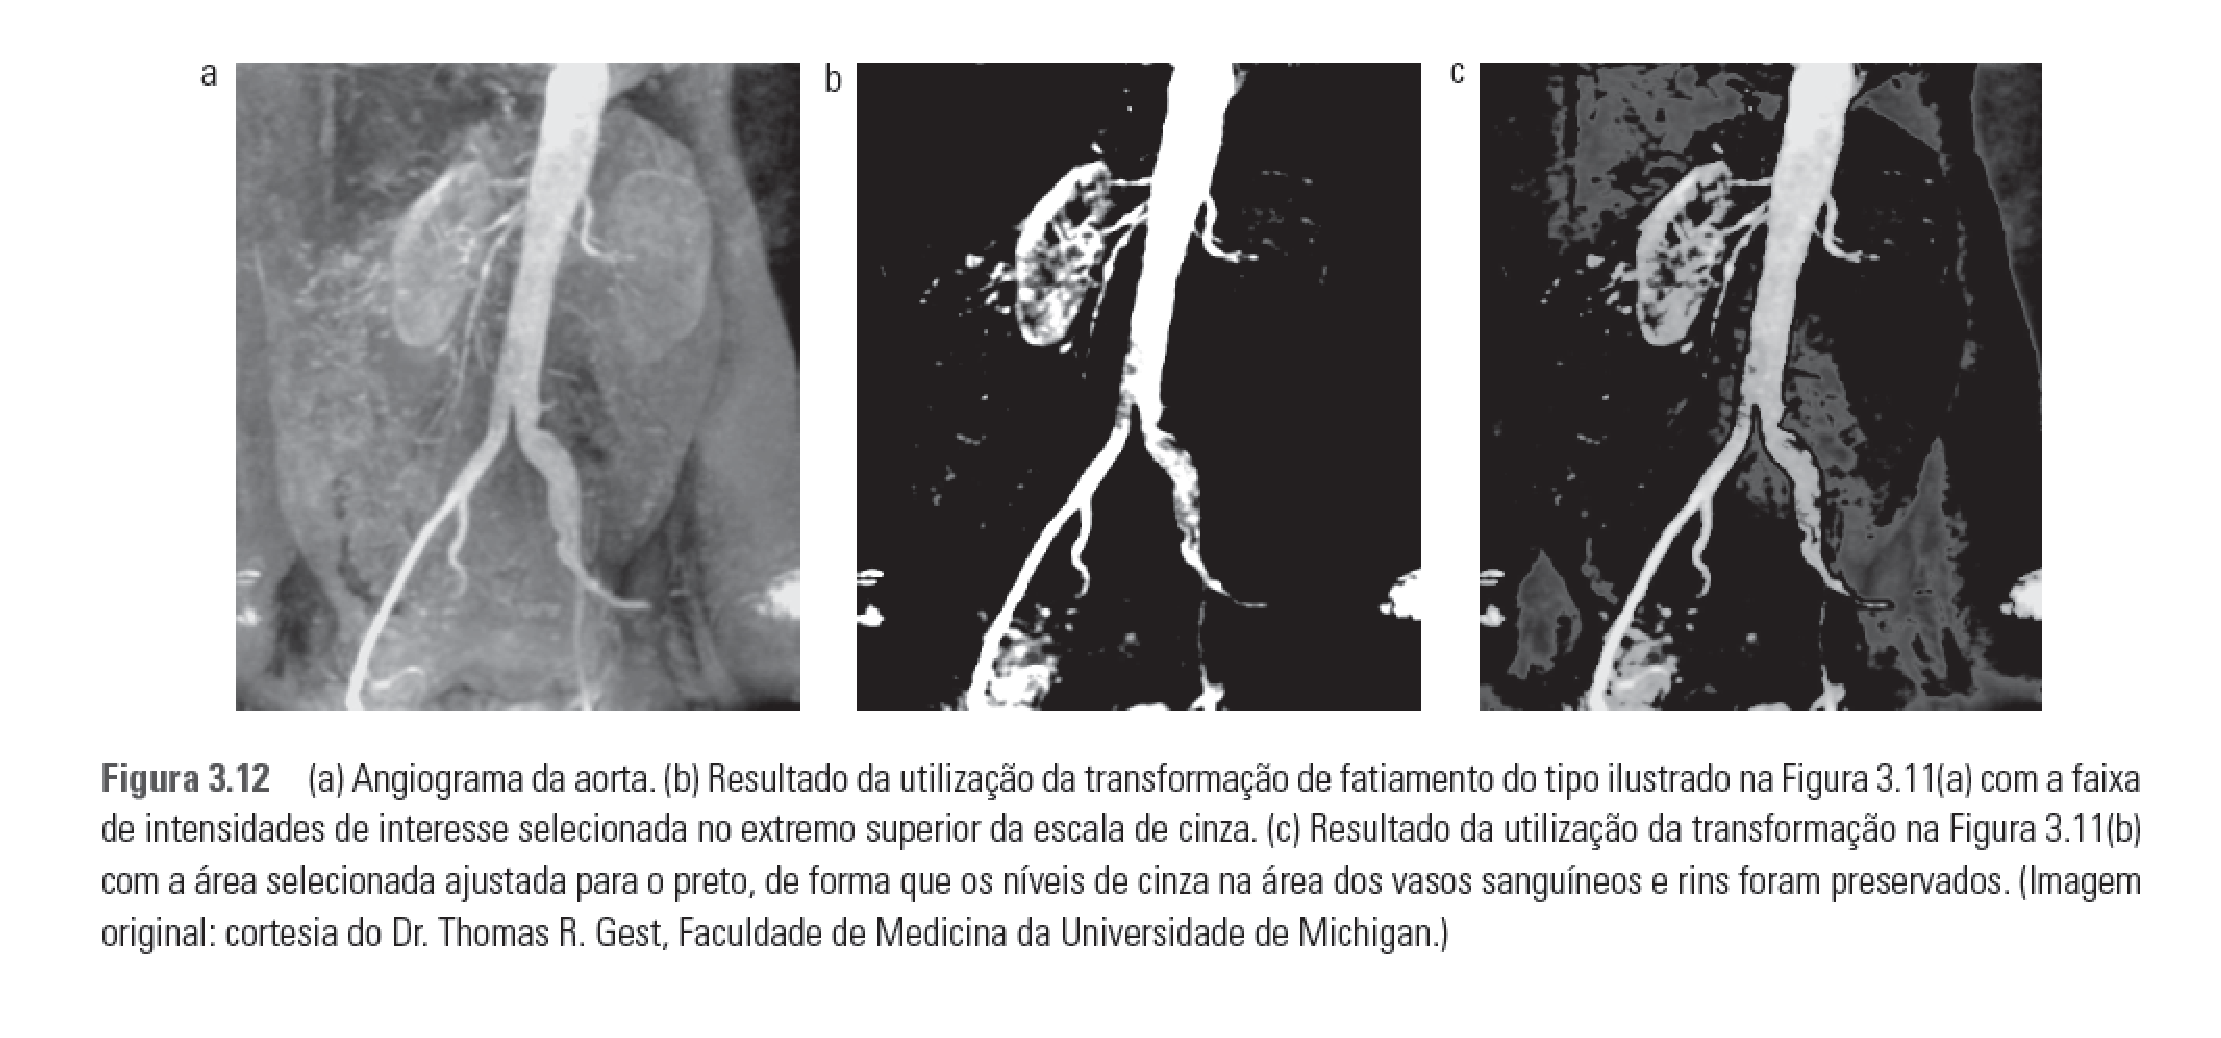
\includegraphics[width=\textwidth]{figs/fig0312}
         \end{center}
    \end{slide}

   \begin{slide}[toc=]{Fatiamento por planos de bits}
      \begin{itemize}
         \item Uma imagem pode ser considerada como composta por planos de bits empilhados
      \end{itemize}
         \begin{center}
             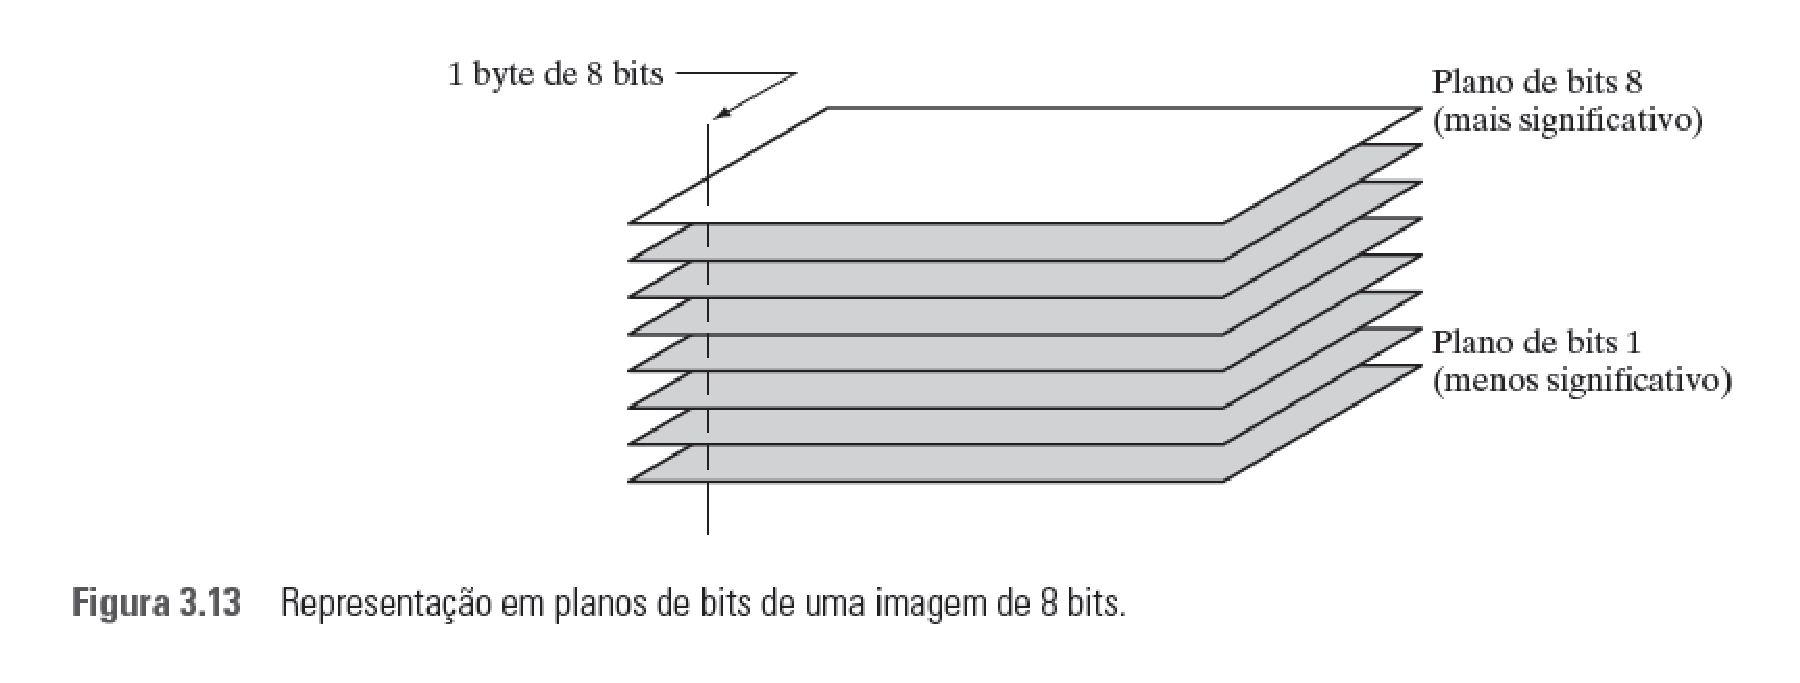
\includegraphics[width=\textwidth]{figs/fig0313}
         \end{center}
    \end{slide}

    \begin{slide}[toc=]{Fatiamento por planos de bits}
      \begin{itemize}
         \item Contribuição de cada plano de bit na formação de uma imagem
      \end{itemize}
         \begin{center}
             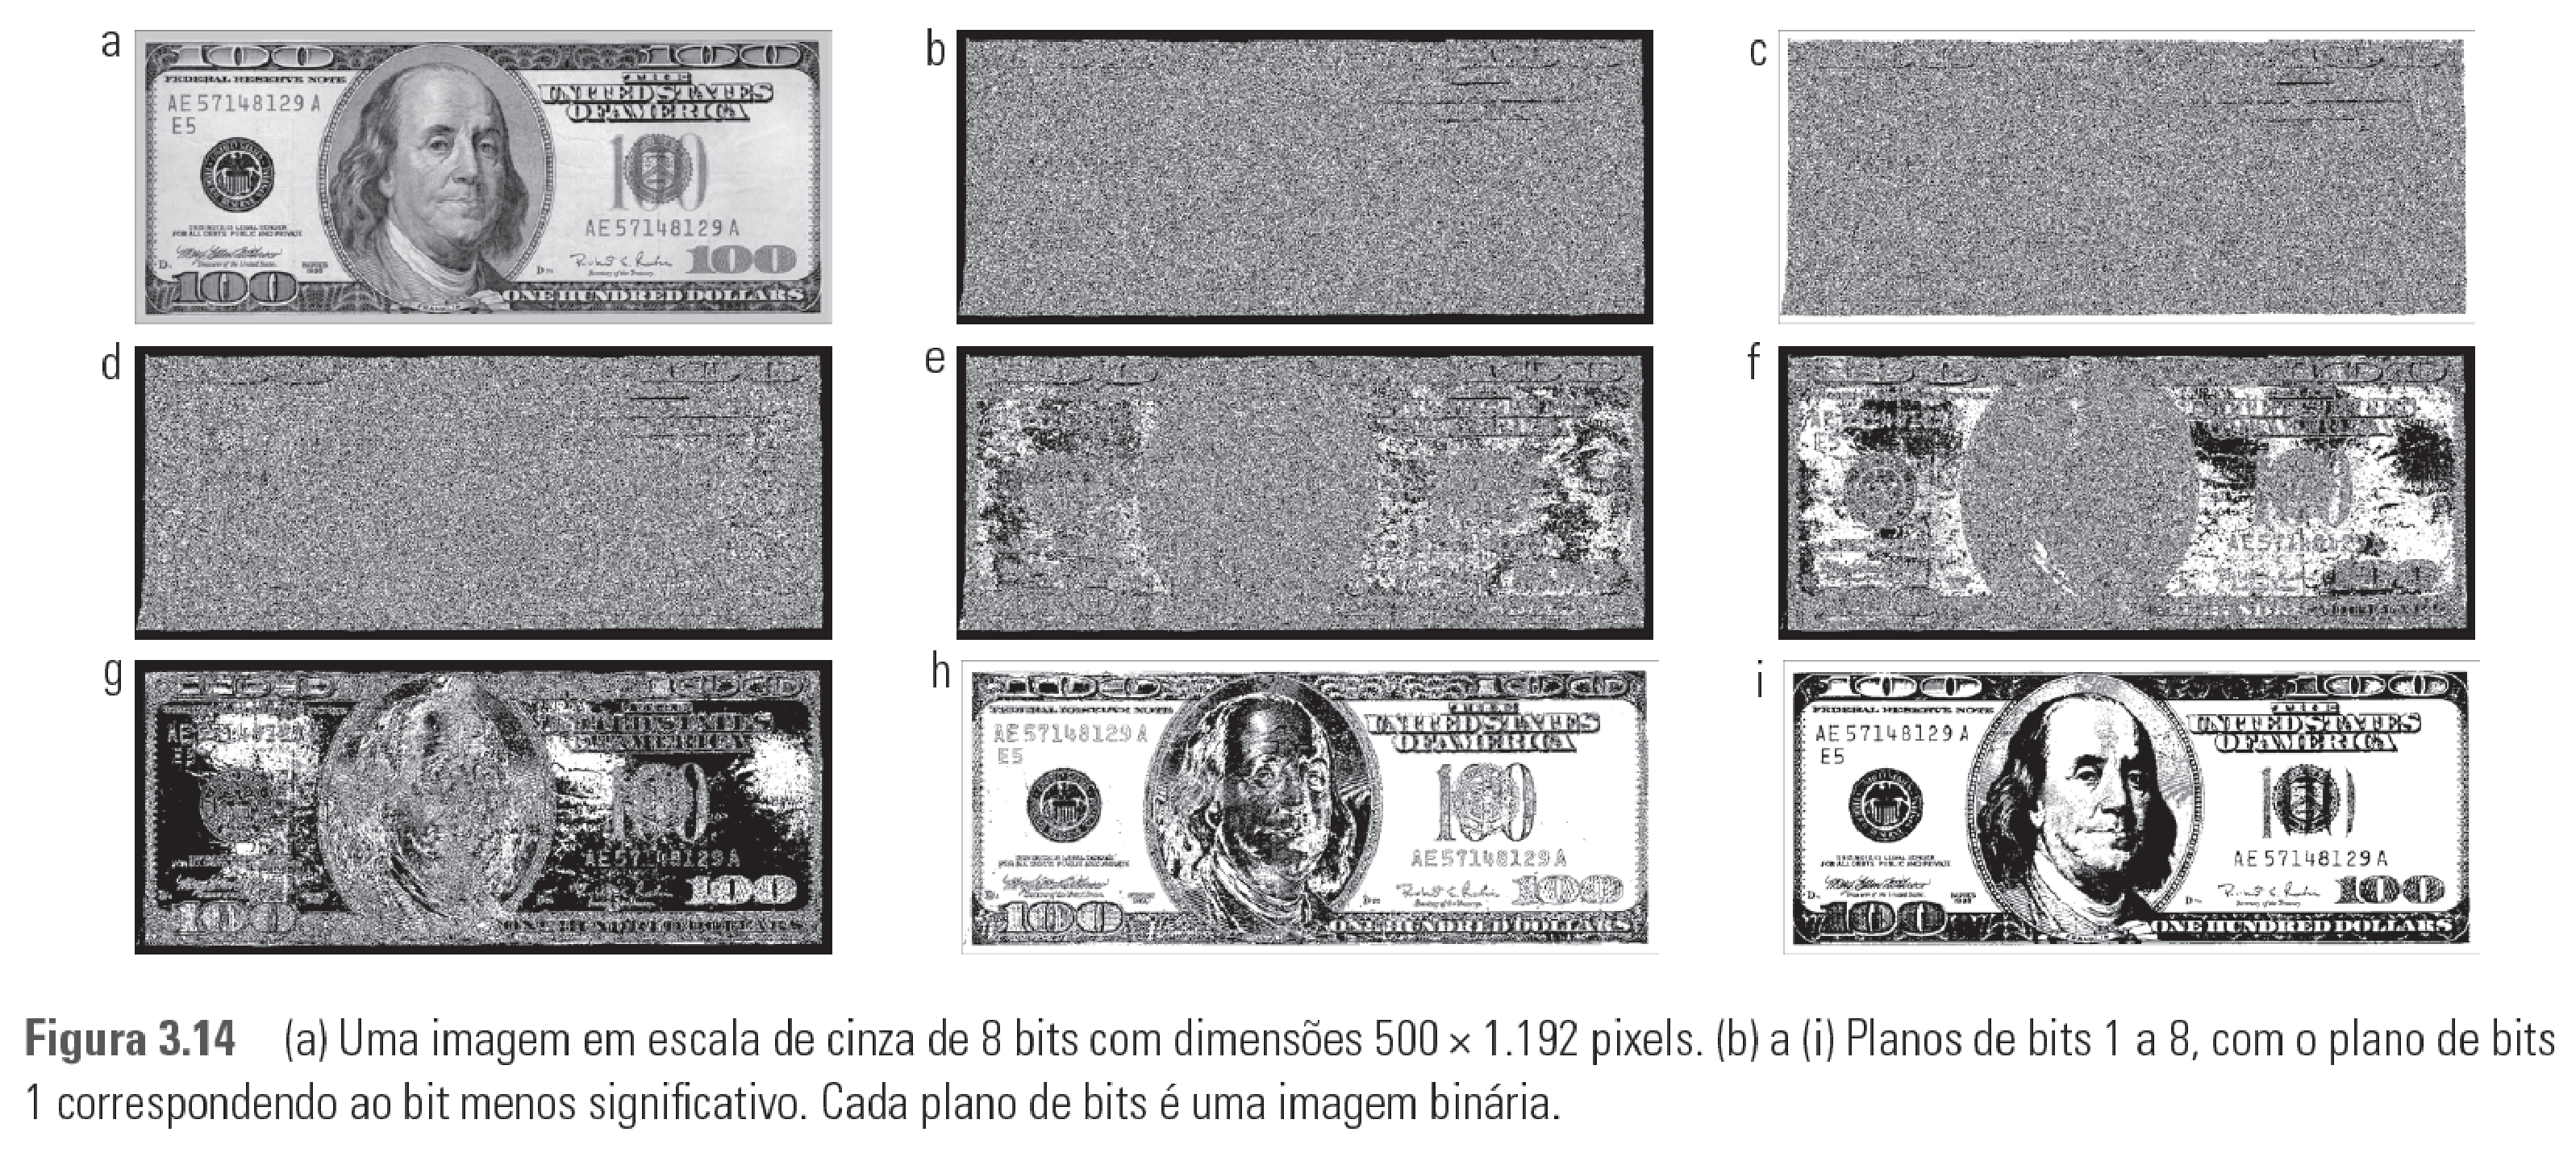
\includegraphics[width=\textwidth]{figs/fig0314}
         \end{center}
    \end{slide}
    
   \section[ slide = true]{Processamento de histograma}
   \begin{slide}[toc=]{Histograma}
      \begin{itemize}[type=1]
         \item Definição
         \begin{equation*}
             p(k) = \frac{n_k}{MN}
         \end{equation*}
         \begin{itemize}
            \item $p$: histograma
            \item $k$: valor de intensidade do pixel
            \item $n_k$: número de pixels de intensidade $k$ em uma dada imagem
            \item $MN$: número total de pixels de uma dada imagem
         \end{itemize}
         \item O histograma pode ser visto como uma estimativa da função de densidade de probabilidade de uma imagem
      \end{itemize}
   \end{slide}

    \begin{slide}[toc=]{Histograma: exemplos}
      \begin{itemize}
         \item Imagens escura e clara
      \end{itemize}
         \begin{center}
             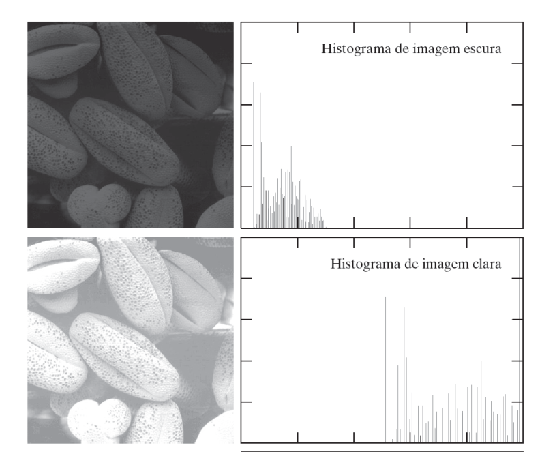
\includegraphics[height=0.65\textheight]{figs/fig0316a}
         \end{center}
    \end{slide}

    \begin{slide}[toc=]{Histograma: exemplos}
      \begin{itemize}
         \item Imagens de baixo e alto contraste
      \end{itemize}
         \begin{center}
             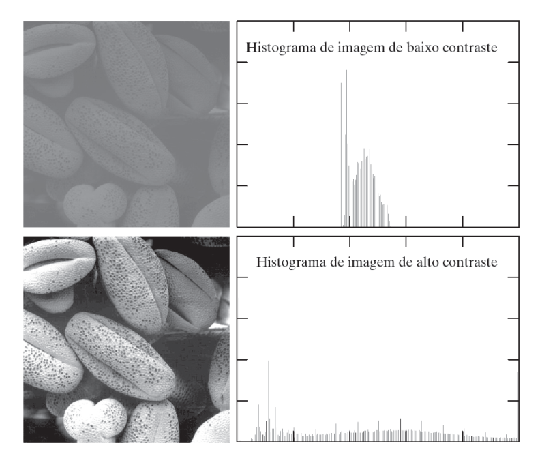
\includegraphics[height=0.65\textheight]{figs/fig0316b}
         \end{center}
    \end{slide}

    \begin{slide}[toc=]{Equalização de histograma}
      \begin{itemize}
         \item O objetivo é obter um \underline{histograma uniforme} (idealmente) no intervalo de intensidades de $0$ a $L-1$
         \begin{center}
             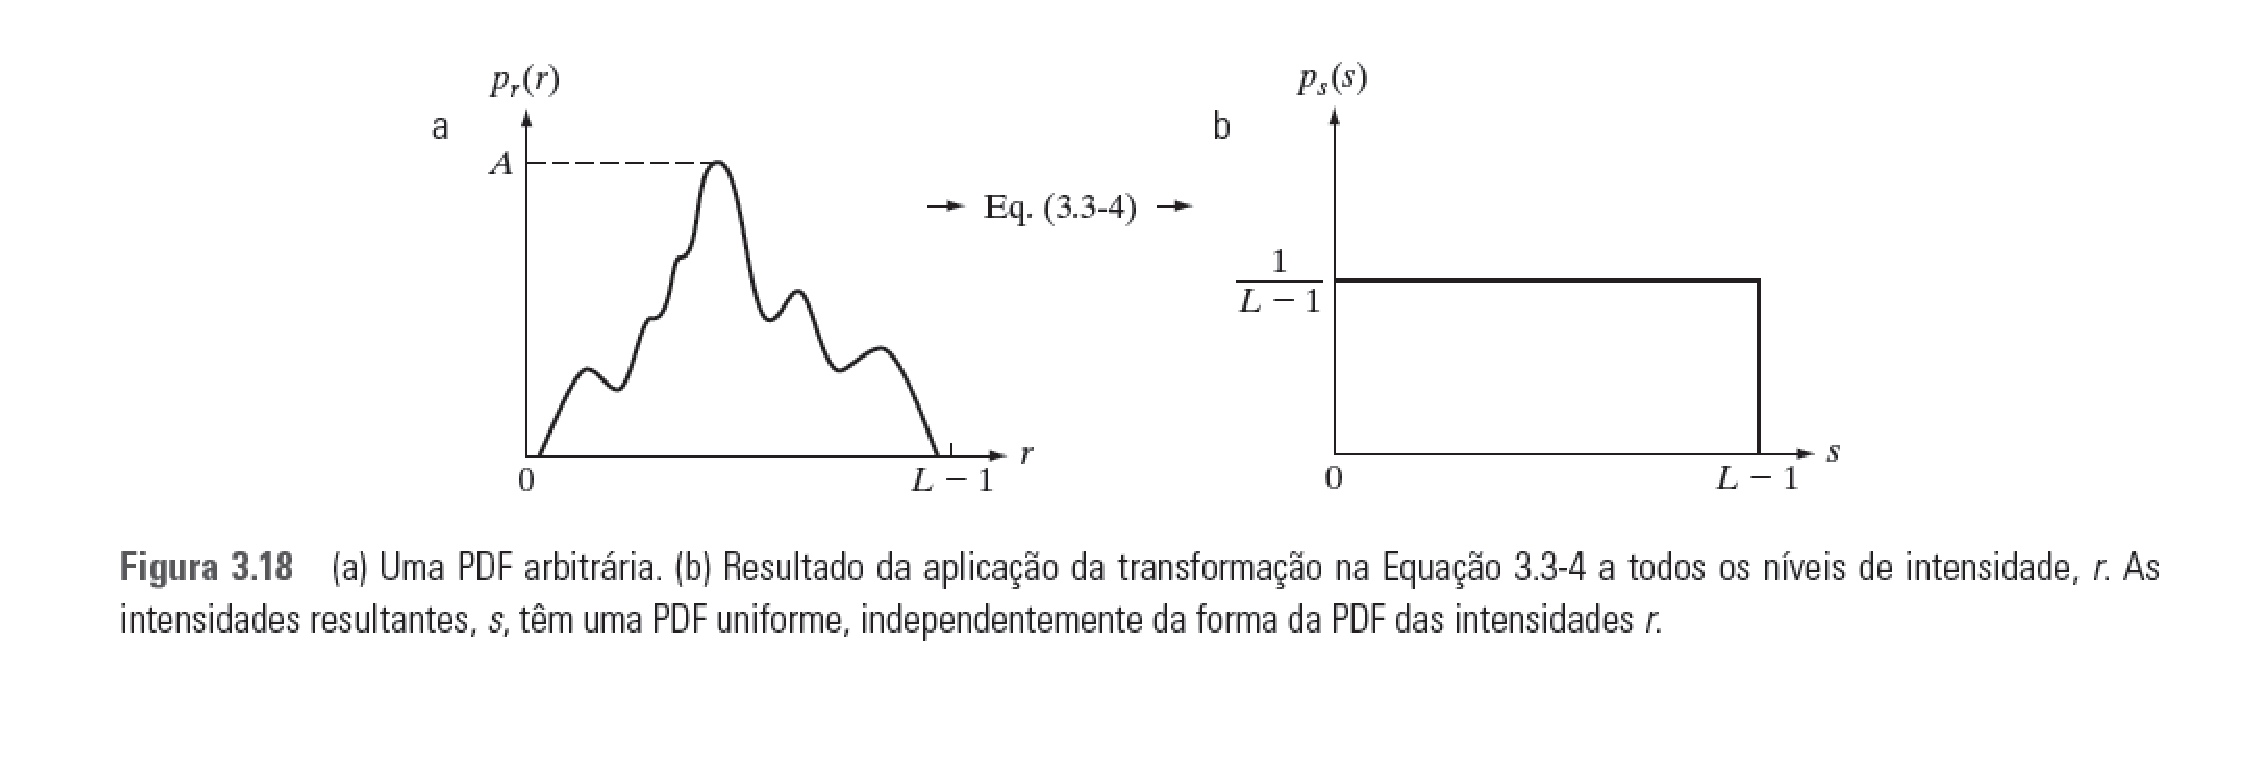
\includegraphics[width=0.9\textwidth]{figs/fig0318}
         \end{center}\pause
         \item \underline{Histograma} como \underline{função de densidade de probabilidade}:
         \begin{itemize}
            \item Como gerar uma variável aleatória de distribuição uniforme a partir de uma variável aleatória de distribuição arbitrária?\pause
             ~Lembrou?
         \end{itemize}
      \end{itemize}
    \end{slide}

    \begin{slide}[toc=]{Equalização de histograma}
      \begin{itemize}
         \item Função de distribuição de probabilidade $F_X(x)$ da variável aleatória $X$ ($X\in [0, L-1]$)
         \begin{align*}
             F_X(x) &=P\{X\leq x\}\\
                    &=\int_{-\infty}^x f_X(\alpha)d\alpha
         \end{align*}
         \begin{itemize}
            \item $f_X(x)$: função de densidade de probabilidade da variável aleatória $X$ (arbitrária)
         \end{itemize}\pause
         \item \underline{Objetivo}: determinar uma função $g(X)$ monotônica, tal que $Y=g(X)$ tenha uma distribuição uniforme:
         \begin{equation*}
             F_Y(y) = \frac{1}{L-1}y
         \end{equation*}

      \end{itemize}
   \end{slide}    


    \begin{slide}[toc=]{Equalização de histograma}
      \begin{itemize}
         \item Sendo $g(X)$ uma função monotônica
         \begin{align*}
             P\{Y\leq y\} &= P\{X\leq x\}\\
                          &= F_X(x)\\
                          &= \frac{1}{L-1}y
         \end{align*}\pause
         \begin{center}
            \fbox{$Y = (L-1)F_X(X)$}
         \end{center}
      \end{itemize}
   \end{slide}    
\end{document}
